\documentclass{article}


\usepackage{graphicx} % Required for inserting images
\usepackage{biblatex} %Imports biblatex package
\usepackage{booktabs} % Required for tables
\usepackage{longtable}
\usepackage{float}
\usepackage{rotating} % Required for sideways table

\addbibresource{references.bib}


\title{Learning to pump in slalom}
\author{Christian Magelssen}
\date{February 2024}


\begin{document}


\section{Introduction}

Developing sporting expertise involves learning to choose and develop good strategies to ensure continuous skill improvement and prevent plateaus. In alpine ski racing, these strategies are intended to ensure that a skier skis a course in the shortest possible time. As long as the skier passes on the correct side of the gates that mark the course, they have the freedom to choose their preferred strategy. This redundancy in the task has sparked considerable interest among skiers, coaches, and scientists in identifying the most effective strategies for ski racing. Understanding these strategies is crucial for training both current and future generations of skiers.

One section of a slalom course where many skiers' performance has not yet reached an asymptote is the flat section of the course. A characteristic feature of this course profile is that the component of gravity pulling skiers down the slope is small, making it key to conserve the available energy as must as possible, such as by executing clean carving turns instead of skidding turns. Improving descending times in this course section solely by minimizing energy dissipation is a conservative strategy. A more offensive strategy involves pumping to increase speed, which, in addition to skiing as cleanly as possible, involves executing additional movements to increase velocity. This move involves extending the center of mass toward the turn's center of rotation. According to a well-known explanatory model, doing this work against the centrifugal force increases the kinetic energy and consequently the velocity coming out of the turn. While the contribution of pumping to overall performance in alpine skiing is debated, it has been observed that elite skiers show surplus kinetic energy in parts of the turn. This surplus energy indicates that..

We have also found evidence that pumping is important for improving race times in slalom skiing. In a five-day learning intervention involving 65 alpine ski racers aimed at enhancing their flat skiing times in slalom using this strategy, we found that athletes on average massively improved their times.


Intervensjonenens hensikt var å teste om trening under hyppig oppgavebytte (interleaved pratice) ga bedre læring enn trening under med liten grad av oppgavebytter (blocked practice). I et stort antall laboratoriestudier har det blitt funnet at interleaved practice gir bedre retention enn blocked practice, selv om generaliseringen av denne til komplekse og mer virkelighetsnære oppgaver er mer tvilsomt. Vi fant heller korreborerende evidens for denne effekten. Derimot fant vi at utøverne forbedret seg massivt på flatene som følge av intervensjonen. På tre av de fem skilagene som deltok brukte satte vi opp lokaltposisjoneringssystem







hyppig oppgavebytte gir bedre læring en lite bytte på motorisk læring, som vi ikke fant overbeviste evidens for. Vi fant riktignok store tidsforskjeller. For tre av skigruppene som vi testet satte vi opp lokalt posisjoneringssystem på baseline og retention for å kunne studere de kinematiske endringene i


 


Et særtrekk for denne løypeprofilen er at komponenten av gravitasjonskraften som trekker utøvere ned en løype er liten som gjør det viktig å ikke sløse med den disponible energien, som for eksempel ved å kjøre rene carvende svinger fremfor skrensende svinger. Å forbedre nedfartstidene i alpint utelukkende gjennom å minimere energitap er en conservativ strategi. En mer offansive strategi er å pumpe for å øke hastighet som i tillegg til å kjøre renest mulig, handler om å utføre tilleggsbevegelser for å øke hastigheten på ski. Denne tilleggsbevegelsen er å pumpe seg til høyere hastighet gjennom å strekke center of mass mot the svingens svingsenter. I en kjent forklaringsmodell bidrar dette arbeidet mot sentrifulalkraften til å øke den kinetiske energien og dermed hastigheten ut av svingen. Selv om det er omdiskutert hvor mye bidrag pumping har å si for den totale prestasjonen i alpint, har det blitt observert at gode alpinister har overskytende kinetisk energi i deler av sving. 

I en 

In a previous study we conducted a large five-day learning experiment on the contextual interference effect in an indoor skiing hall where skilled ski racers trained the pumping technique. To improve this technique we gave the skiers a short introduction of the pumping technique supported by theoretical explanation of its mechanics as well as videos with elite skiers demonstrating this skill. Although we did not find convincing evidence for the contextual interference effect, the skiers improved their flat section massively, suggesting that the pumping technique can be an important skill.













The rider can pump hirns elf and the
cart to a higher velocity if anywhere in his transit of a curve he pushes
his center of mass toward the center of that curve.


In alpine skiing, these strategies revolve around navigating a slalom course as quickly as possible. As long as the skier passes on the correct side of the gates that mark the course, they have the freedom to choose their preferred strategy. This redundancy in the task has sparked considerable interest among skiers, coaches, and scientists in identifying the most effective strategies for ski racing. Understanding these strategies is crucial for training both current and future generations of skiers 



In alpine ski racing, the goal is to ski a course in the shortest time possible. Denne målet kan oppnås ved hjelp av mange ulike strategier så lenge utøveren passerer på riktig side av portene som [make up the course]. 




Developing sporting expertise involves learning to choose and develop good strategies to ensure continuous skill development and prevent plateaus. I alpint skikjøring er det mange løsninger 




The regulations in alpine ski racing allow a broad range of such strategies, as long as the skier passes the correct side of the gates that make up a slalom course. 


Å frigjøre sportslig fremragende krever valg av gode strategier for å hjelpe utøvere med å overvinne platåer og oppnå suksess 




Unleashing sporting excellence requires selection of good strategies to help athletes overcome plateaus and attain success. In alpine ski racing, these 


requires selection of good strategies to help athletes overcome plateaus and attain success. The regulations in alpine ski racing allow a broad range of such strategies, as long as the skier passes the correct side of the gates that make up a slalom course. Due to the redundancy of this sporting task, there has been great engagement among skiers, coaches and scientists in uncovering the underlying strategies for effective ski racing to use this knowledge to train the current and next generation of skiers \cite{joubertHowSkiNew1967, joubertSkiArtTechnique1978, mullerAnalysisBiomechanicalCharacteristics1994, lemasterSkierEdge1999, lemasterUltimateSkiing2010}.

One section of a slalom course where performance has not yet asymptoted for many skiers is the flat section of slalom course. In this section of the course, the component of the gravity vector that propels the skiers down the course is low, which changes what an effective strategy is for this section. One way to ski effectively in this section is to use the "pumping to increase velocity" technique, which is described as extending the body around the. This effect has been observed in many skilled and elite skiers in various disciplines and course.

In a previous study we conducted a large five-day learning experiment on the contextual interference effect in an indoor skiing hall where skilled ski racers trained the pumping technique. To improve this technique we gave the skiers a short introduction of the pumping technique supported by theoretical explanation of its mechanics as well as videos with elite skiers demonstrating this skill. Although we did not find convincing evidence for the contextual interference effect, the skiers improved their flat section massively, suggesting that the pumping technique can be an important skill.

Before and after the skiers underwent the intervention, we recorded the skiers positions with local positioning system while they skied the slalom course. This data can be informative to understand more closely how the skiers improved their race times. Our question was if some these... To examine this question we estimated the mean differences in velocity and accelerations using multilevel Generalized Additive Models (GAMs).

\subsection{Results}


\begin{figure}[H]
\centering
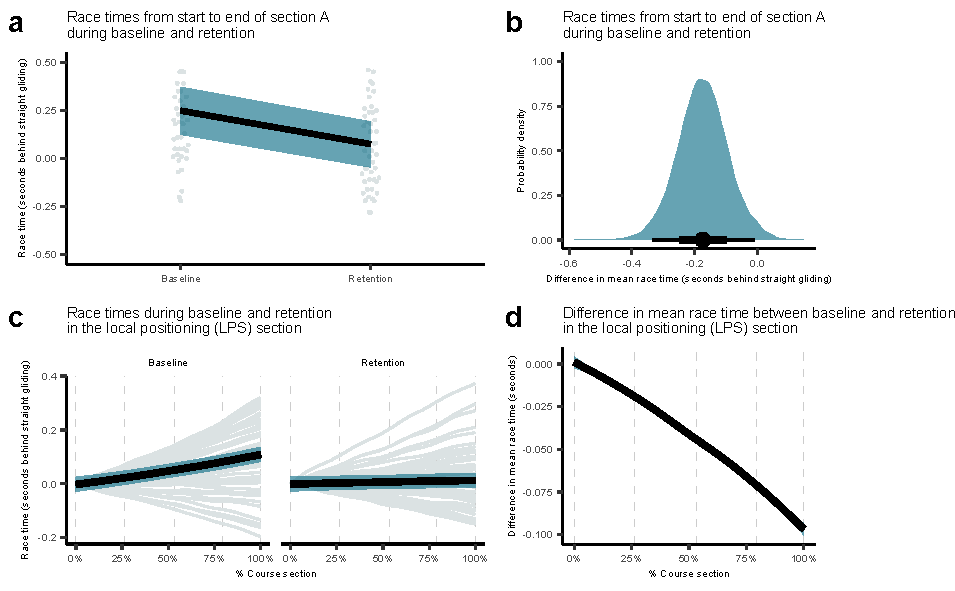
\includegraphics{figurer/figure_racetime.pdf}
\caption{Strategy selection for reinforcement learning (red) and supervised (free choice) learning (blue) during acquisition.}\label{fig: choice_estimated}
\end{figure}


\subsection{Race time}
As a first step we analyzed the intermediate times retrieved from the timing system and the times measured by the local positioning system in the section it covered. This step was necessary to ensure that the race time improvement reported our previous study could be traced all the way back to the upper part of the course and therefore form the basis for further kinematic analyses to explain this improvement. 


Figure \ref{fig: choice_estimated}a viser tidene fra tidtakersystemet fra baseline og retention. Vi fant at utøverne i snitt forbedret sine renntider med -0.17 (95\% CI[-0.33, 0.01])  (Figure \ref{fig: choice_estimated}b fra baseline). Merk at disse tidene dekker seksjonen fra start til litt etter der det lokale posisjoneringsystemer slutter å måle.


Figure \ref{fig: choice_estimated}a viser tidene fra tidtakersystemet fra baseline og retention. Vi fant at den gjennomsnittlige forbedringen var på  -0.17 og CI (-0.33, -0.01), figur \ref{fig: choice_estimated}b. Det er dermed grunnlag for å tro den analyserte sekvensen kan være aktuell for videre analyser.


\section{Metode}


\subsection*{Participants}
This study's sample comprised eighteen alpine ski racers (age M = 16.7 years, SD= 1.1; 7 females, 11 males) from three development ski academies in Norway. The eighteen skiers composed a subset of a larger sample (64 skiers) from which we already published results. The reason for this subsetting was because we only used local positioning system at the upper section of the course for this group of skiers. Except for three skiers, all participants had competed in Fédération International de Ski (FIS) races, and FIS points were recorded (\textit{M} = 115, \textit{SD}=31) in slalom. However, it is worth noting that their FIS points poorly reflect the skiers' skill levels owing to the difficulty in organizing races during the COVID-19 pandemic, which decreased the opportunities to collect points.  

\subsection{Setup}

The experiment was conducted on a 250-meter-long flat section of the race hill at the indoor ski hall SNØ, Norway. In this section, we sat three slalom courses to tease the contextual interference effect. Course B, from which the data for this study are reported, was the middle of the three courses and had a 1.7-meter gate offset with a 10-meter vertical distance. This course dimension was the most typical of the three courses and was one of the reasons we selected this course only. Before each ski team tested, water was injected into the hill to create an icy yet grippy snow layer.

To occlude variation in starting procedures to cause variation in times, we used a standardized starting procedure. The skiers started 20 meters before the first gate and started from a stationary position with the ski bindings behind the start gate. When allowed clearance to start, the skiers lifted the poles up from the snow and skied straight down 10 meters from the hill until they crossed the first photocell that initiated the timer. After this, the skiers could ski normal. For this study, a trial ended when the skiers crossed the second intermediate time, but the skiers continued the rest of the course. We recorded the times using a wireless photocell timing system (HC Timing wiNode and wiTimer; Oslo, Norway).

In a shorter section of this area, we set up a local positioning system (LPS) consisting of three nodes on each side of the track. One of these nodes served as the master node and was positioned on the skier's right side of the track. This local positioning system provided positional data from the skiers as they descended the course section. With these data, we were able to calculate the velocity and acceleration of the skier. Originally, our intention was to track the skiers using the local positioning system from the beginning to the end of the sequence. However, we encountered signal challenges in the upper part of the ski hall due to its narrow width. Similar disturbances are commonly associated with the local positioning system when nodes are placed too close to walls. As a result, we had to filter the local positioning system data to focus solely on the sequence between the last five gates in the local positioning system section.

\subsection{Design and procedure}
In the original study, we employed a between-subject design where skiers were allocated to either an interleaved group or a blocked group. The interleaved group skied all slalom courses on the same day in an interleaved order, while the blocked group completed only one of the three courses per day. Further specifics can be found in the original study. Since we did not find evidence for the contextual interference effect in this study, we have chosen to omit this group information in the modeling work, and henceforth, we only describe the procedure.

Figure provided an illustrative overview of the experimental procedure. The baseline tests began with two warm-up rounds. One consisted of free skiing down the race hill, while the other involved a specific warm-up within one of the race courses. Following this, skiers completed a run straight down the course in a static, upright position, serving as a reference to account for variations in snow and section length. Subsequently, skiers completed a total of 12 rounds, three of which were within the same course we are reporting on in this study (course B). Midway and after these 12 rounds, a new straight gliding run was performed. The one in the middle was randomly placed for each skiers.

 






Baselinetesten begynte med to oppvarmingsrunder hvorav en var ren frikjøring i renntraseen mens den andre var en spesifikk oppvarming i løypen. Deretter fullførte utøverne en runde der de kjørte løypen rett ned i en statisk, oppreist posisjon. Hensikten med denne nedkjøringen var for å ha en referanse som tok hensyn til variasjon i underlag. Deretter utførte utøverne totalt 12 runder hvorav tre var i løypen som vi rapporterer fra i denne studien. Midtveis og etter denne denne økten fullførte en ny straight gliding runde. Den i midten ble tilfeldig plassert for hver utøver.

Etter baselinetesten samlet vi utøverne for en gjennomgang av pumpeteknikken hvor vi la frem teoretisk forklaring og evidens fra World Cup som viser denne effekten. Utøverne ble forklart at de skulle strekke seg så mye de kunne inn mot svingens rotasjonssenter. Deretter ble utøverne allokert i de to gruppene.

Tilegnelsenfasen bestod av tre dager med øving på pumpeteknikken med tidene (uttrykt som forskjellen fra straightgliding) som tilbakemelding. Hver økt bestod av totalt 12 runs on the three courses, hvorav den første og siste runden var en straight gliding tid. 

Retention testen ble gjennomført 72 timer etter siste økt under tilegnelsesfasen. Her fikk heller ikke utøverne få vite tidene sine. 



\subsection{Analysis}


All calculations were conducted in Matlab with available scripts developed, tested, and used for previous studies \cite{reidKinematicKineticStudy2010}. The files were then imported into Python using the  \cite{2020SciPy-NMeth} and pandas \cite{reback2020pandas} package. However, some runs were not part of the experimental protocol, such as warm-up runs or freeskiing, which caused trouble importing to Python. In addition, in a few cases, the quality of the local positioning signal was deficient, so the calculations in Matlab could not proceed. In both situations, the runs were manually dropped from the Matlab file. All manually dropped runs are reported in document A. The remaining data underwent two manual screening processes to check and confirm the quality of the local positioning data. The first screening process was to remove all runs that did not match the experimental procedure, such as warm-up runs or run numbers where we had recorded a Did Not Finish (DNF). In the second screening process, we visually inspected all runs to detect errors in the local positioning data. To help with this detection, we plotted section time performance, coordinates, and velocity for all ski racers. All removed runs, including the reasons for removal, are reported in document A. Finally, the data that passed the screening process was entered into a MySql database.



\end{document}
